%%%%%%%%%%%%%%%%%%%%%%%%%%%%%%%%%%%%%%%%%%%%
% En 'includes.tex' se encuentran la importación de paquetes necesarios
%%%%%%%%%%%%%%%%%%%%%%%%%%%%%%%%%%%%%%%%%%%%
%%%%%%%%%%%%%%%%%%%%%%%%%%%%%%%%%%%%%%%%%
% University Assignment Title Page 
% LaTeX Template
% Version 1.0 (27/12/12)
%
% This template has been downloaded from:
% http://www.LaTeXTemplates.com
%
% Original author:
% WikiBooks (http://en.wikibooks.org/wiki/LaTeX/Title_Creation)
%
% License: CC BY-NC-SA 3.0 (http://creativecommons.org/licenses/by-nc-sa/3.0/)
% 
% Instructions for using this template:
% This title page is capable of being compiled as is. This is not useful for 
% including it in another document. To do this, you have two options: 
%
% 1) Copy/paste everything between \begin{document} and \end{document} 
% starting at \begin{titlepage} and paste this into another LaTeX file where you 
% want your title page.
% OR
% 2) Remove everything outside the \begin{titlepage} and \end{titlepage} and 
% move this file to the same directory as the LaTeX file you wish to add it to. 
% Then add \input{./title_page_1.tex} to your LaTeX file where you want your
% title page.
%
%%%%%%%%%%%%%%%%%%%%%%%%%%%%%%%%%%%%%%%%%
%\title{Title page with logo}
%----------------------------------------------------------------------------------------
%	PACKAGES AND OTHER DOCUMENT CONFIGURATIONS
%----------------------------------------------------------------------------------------
\PassOptionsToPackage{warn}{textcomp}
\documentclass[14pt]{extarticle}
%Paquetes para idioma español y codifcación UTF8
\usepackage[spanish]{babel}
\usepackage[utf8]{inputenc}
\usepackage{csquotes}

%%% BIBLATEX
\usepackage{biblatex}
%%% BIBLIOGRAPHY
\addbibresource{references.bib}

%fuente 'fourier'
\usepackage{fourier}
%paquete para URLs
\usepackage{url}
\usepackage[hidelinks]{hyperref}
%paquete para ubicar las imágenes
\usepackage{float}
%paquete para imágenes y en dónde las tiene que buscar
\usepackage{graphicx}
\graphicspath{{images/}}
%paquete para epígrafes
\usepackage{subcaption}
%paquete para definir los márgenes de la hoja
\usepackage[left=1.5cm,right=1.5cm,top=3cm,bottom=3cm]{geometry}
%paquete para poner todos y comentarios
\usepackage[colorinlistoftodos]{todonotes}
%paquete para trabajar con código
\usepackage{listings}
%paquete para trabajar con colores y definir propios
\usepackage{color}

%paquete para el checkmark y la cruz
\usepackage{pifont}
%paquete para el signo de copyright
\usepackage{textcomp}

%paquete para que los \texttt{} no rompan el margen de la página
\usepackage[htt]{hyphenat}

\usepackage{enumerate}
%paquete para armar layouts multicolumna
\usepackage{multicol}


%Cabeceras
\usepackage{fancyhdr}
\pagestyle{fancy}
\fancyhead[L]{Administración de Redes y Seguridad, 2018}
\fancyhead[C]{}
\fancyhead[R]{UNPSJB}

\fancyfoot[R]{Luciano Serruya Aloisi}

%Comando para poner doble comillas más fácil
\newcommand{\dq}[1]{``#1''}
\newcommand{\cmark}{\ding{51}}
\newcommand{\xmark}{\ding{55}}

\definecolor{comment-green}{rgb}{0,0.5,0}
\definecolor{bg-light-gray}{HTML}{E9E9E9}
\definecolor{bg}{HTML}{D0B698}

\lstdefinestyle{bashstyle}{
    language=Bash,
    backgroundcolor=\color{bg},
    basicstyle=\ttfamily,
  	keywordstyle=\bfseries\color{white},
    stringstyle=\color{blue},
    commentstyle=\color{comment-green}\itshape,
    numberstyle=\color{gray},
    identifierstyle=\color{black},
    rulecolor=\color{gray},
    showstringspaces=false,
    escapeinside={\%*}{*)},
    morekeywords={},
    otherkeywords={},
    breaklines=true,
    frame=trbl, 
    framexleftmargin=25pt,
    numbers=left,
    xleftmargin=\parindent,
    frameround=tttt,
    captionpos=b,
    % re tirado de los pelos, pero es lo que hay
    % sacado de:
    % https://tex.stackexchange.com/questions/24528/having-problems-with-listings-and-utf-8-can-it-be-fixed
    inputencoding=utf8,
    extendedchars=true,
    literate={á}{{\'a}}1 {é}{{\'e}}1 {í}{{\'i}}1 {ó}{{\'o}}1 {Ó}{{\'O}}1 {ú}{{\'u}}1,
}



\begin{document}

%%%%%%%%%%%%%%%%%%%%%%%%%%%%%%%%%%%%%%%%%%%%
% En 'titlepage.tex' se encuentra la página de título
%%%%%%%%%%%%%%%%%%%%%%%%%%%%%%%%%%%%%%%%%%%%
\begin{titlepage}

    \newcommand{\HRule}{\rule{\linewidth}{0.5mm}} % Defines a new command for the horizontal lines, change thickness here

    \center % Center everything on the page
     
    %----------------------------------------------------------------------------------------
    %	HEADING SECTIONS
    %----------------------------------------------------------------------------------------

    \textsc{\LARGE UNPSJB}\\[1cm] % Name of your university/college
    \textsc{\Large Licenciatura en Sistemas OPGCPI}\\[0.5cm] % Major heading such as course name
    \textsc{\large Administración de Redes y Seguridad}\\[0.5cm] % Minor heading such as course title

    %----------------------------------------------------------------------------------------
    %	TITLE SECTION
    %----------------------------------------------------------------------------------------

    \HRule \\[0.4cm]
    {\huge \bfseries Trabajo Práctico 1}\\[0.4cm] % Title of your document
    {\large \bfseries Concientización}\\[0.4cm] % Title of your document
    \HRule \\[1.5cm]
     
    %----------------------------------------------------------------------------------------
    %	AUTHOR SECTION
    %----------------------------------------------------------------------------------------


    \begin{minipage}[l]{0.5\textwidth}
        \begin{flushleft}
            \textbf{\textsf{Cátedra}}\\
            \large Lic. Bruno Damián Zappellini\\ 
            \linespread{4}
            \end{flushleft}
    \end{minipage}
    \begin{minipage}[l]{0.4\textwidth}
        \begin{flushright}
            \textbf{\textsf{Integrantes:}}\\
            \linespread{1}
            \large Luciano Serruya Aloisi\\
        \end{flushright}
    \end{minipage}\\[1.5cm]

    % If you don't want a supervisor, uncomment the two lines below and remove the section above
    %\Large \emph{Author:}\\
    %John \textsc{Smith}\\[3cm] % Your name

    %----------------------------------------------------------------------------------------
    %	DATE SECTION
    %----------------------------------------------------------------------------------------

    {\large \today}\\[1cm] % Date, change the \today to a set date if you want to be precise

    %----------------------------------------------------------------------------------------
    %	LOGO SECTION
    %----------------------------------------------------------------------------------------

    
\includegraphics[scale=1]{logoUnpsjb.png}\\[0.5cm] % Include a department/university logo - this will require the graphicx package
     
    %----------------------------------------------------------------------------------------

    % \vfill % Fill the rest of the page with whitespace

\end{titlepage}


%%%%%%%%%%%%%%%%%%%%%%%%%%%%%%%%%%%%%%%%%%%%
% INDICE
%%%%%%%%%%%%%%%%%%%%%%%%%%%%%%%%%%%%%%%%%%%%
\clearpage
\tableofcontents
\clearpage 

\lstset{style=bashstyle}

\section{Sistema de autenticación de SSH}

Según las páginas \texttt{man}, el comando \texttt{ssh-keygen} \emph{genera, gestiona, convierte, y autoriza claves para ssh. ssh-keygen puede generar claves para que las use SSH protocolo versión 2} 

\begin{figure}[H]
    \centering
    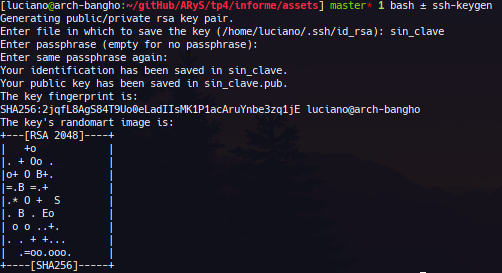
\includegraphics[scale=0.6]{images/ssh-sin-clave.png}
    \caption*{Creación de una llave SSH sin contraseña}
\end{figure}

\begin{figure}[H]
    \centering
    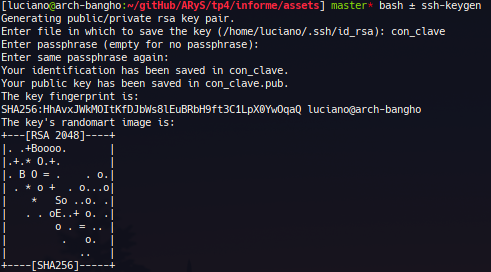
\includegraphics[scale=0.6]{images/ssh-con-clave.png}
    \caption*{Creación de una llave SSH con contraseña \dq{unaClave}}
\end{figure}

\subsection{Archivos de autorización}

Para gestionar el ingreso con \emph{clave pública} y para llevar registro de los sitios confiables a los cuales ya se ingresó, SSH mantiene dos archivos, respectivamente:

\begin{itemize}
    \item \emph{authorized\_keys}: lleva registro de las claves públicas aceptadas para conectarse vía SSH al sistema. Se podrán conectar con autenticación de clave pública sólo aquellos usuarios que tengan la correspondiente clave privada de la clave pública registrada en el archivo 
    \item \emph{known\_hosts}: indica a los sitios que se conectó el usuario y son seguros (antes de establecer la conexión SSH con un sitio nuevo, el sistema pregunta si desea confiar en el sitio) 
\end{itemize}

\subsection{Ingresando a un servidor remoto con clave pública}

Luego de registrar la clave pública personal en el servidor remoto y de haber configurado este último para que sólo permita ingresar (por SSH) mediante clave pública, se puede ingresar al servidor sin problemas.

Gracias al \emph{log} que imprime SSH al ejecutarlo con la bandera \texttt{-vvv}, se puede ver la siguiente sección con respecto al ingreso con clave pública

\begin{lstlisting}
.
.
.
debug1: Authentications that can continue: publickey
debug3: start over, passed a different list publickey
debug3: preferred publickey,keyboard-interactive,password
debug3: authmethod_lookup publickey
debug3: remaining preferred: keyboard-interactive,password
debug3: authmethod_is_enabled publickey
debug1: Next authentication method: publickey
.
.
.
\end{lstlisting}

\section{Túneles}










%%%%%%%%%%%%%%%%%%%%%%%%%%%%%%%%%%%%%%%%%%%%
% FIN DOCUMENTO, AHORA REFERENCIAS
%%%%%%%%%%%%%%%%%%%%%%%%%%%%%%%%%%%%%%%%%%%%
\clearpage
\printbibliography

\end{document}
